% !TEX encoding = UTF-8
% !TEX TS-program = pdflatex
% !TEX root = ../tesi.tex

%**************************************************************
\chapter{Progettazione e codifica}
\label{cap:progettazione-codifica}
%**************************************************************

\intro{Questo capitolo presenta lo studio della parte di interesse del framework aziendale e l'attività di progettazione svolta per il progetto, approfondita con diagrammi UML. La progettazione viene organizzata in due parti: progettazione dell'estensione del framework e progettazione dell'applicazione, per mantenere separate le due parti di software prodotte durante lo svolgimento dello stage. La progettazione è avvenuta seguendo un approccio top-down: dapprima sono state individuate le componenti ad alto livello e la loro interazione, fino all’individuazione dei singoli moduli e delle classi.}\\

%**************************************************************
\section{Premessa: architettura e funzionamento \\ del framework}
\begin{figure}[!h]
    \begin{widepage}
        \label{fig51}
        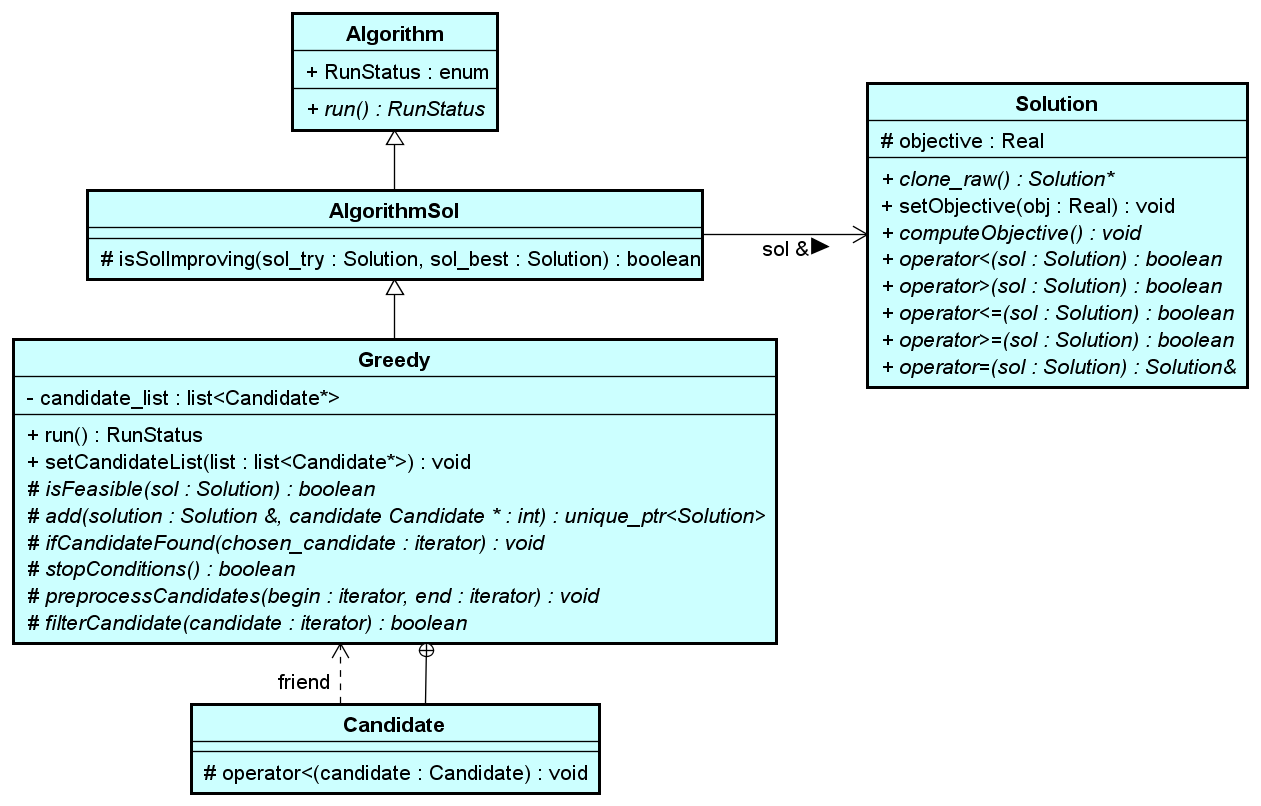
\includegraphics[width=14.9cm,keepaspectratio]{../immagini/progettazione/framework.png}
        \caption{Architettura di dettaglio di parte del framework aziendale}
    \end{widepage}
\end{figure}
Il framework aziendale, come già accennato, offre una base per l'implementazione di algoritmi di ottimizzazione e consiste di librerie per l'utilizzo di grafi, di algoritmi euristici di tipo greedy e di meta-euristiche, ad esempio Tabu Search. 
Per l'estensione del framework con la risoluzione dei problemi di scheduling, durante lo stage ho dovuto utilizzare la parte di libreria atta all'implementazione di algoritmi greedy; di seguito ne viene riportata la sua struttura e ne sono messi in evidenza i metodi di interesse. L'architettura è mostrata in \hyperref[fig51]{Figura 5.1}.
\paragraph{Algorithm} la classe \texttt{Algorithm} è un'interfaccia per l'implementazione di qualsiasi algoritmo. Ha un unico metodo virtuale puro, \texttt{run()}, che deve essere implementato nelle sue classi derivate con il corpo dell'algoritmo di risoluzione; esso deve ritornare un \texttt{RunStatus}: SUCCESS\textunderscore RUN, FAIL\textunderscore RUN, UNFEASIBLE.
\paragraph{AlgorithmSol} è derivata da \texttt{Algorithm} ma ancora astratta in quanto non dà un'implementazione del metodo \texttt{run()}. Essa rappresenta un ulteriore strato prima di poter implementare gli algoritmi, in quanto contiene un riferimento alla classe \texttt{Solution}. Il suo unico metodo \texttt{isSolImproving()} serve a confrontare gli objective di due \texttt{Solution} per stabilire quale delle due sia la migliore.
\paragraph{Candidate} è interna a \texttt{Greedy} e rappresenta un candidato da valutare all'interno del metodo \texttt{run()}. Va estesa con classi derivate che aggiungano le strutture dati. Una lista di tutti i candidati è campo dati di \texttt{Greedy}.
\paragraph{Greedy} è derivata di AlgorithmSol e rappresenta un template di implementazione per gli algoritmi greedy. Implementa il metodo \texttt{run()} con uno ``scheletro'' generale valido per tutti gli algoritmi di tipo greedy, applicando il \emph{\gls{design}}\glsfirstoccur\ ``Template Method''. Tutti gli altri metodi virtuali rappresentano gli hook per il metodo template e devono essere implementati nelle classi derivate a seconda di che algoritmo greedy si vuole implementare.
\paragraph{Solution} è una classe astratta che rappresenta la soluzione trovata all'interno del metodo \texttt{run()}. Ha come unico campo dati \texttt{objective}, che è il risultato della funzione obiettivo implementata dentro il metodo virtuale puro \texttt{computeObjective()}. Nelle classi derivate bisogna implementare tale metodo, gli operatori di confronto, e aggiungere una struttura dati che permetta di mantenere memoria della soluzione.

\subsection{Il metodo run()}
Essendo il punto cardine dell'estensione del framework, è opportuno spiegare il funzionamento del metodo template \texttt{run()} implementato all'interno di \texttt{Greedy}. A tale scopo se ne riporta uno pseudocodice estremamente semplificato, con i metodi virtuali puri da implementare nelle classi derivate evidenziati in rosso:
\newpage
\begin{lstlisting}
while(!stopConditions()){
    preprocessCandidates(list_begin, list_end);
    chosen_candidate =list_end;
    list<Candidate*>::iterator candidate;
    for (candidate = list_begin; candidate != list_end; candidate++){
        if (filterCandidate(candidate))
            continue;
        solution_try = add(sol, candidate);
        solution_try.computeObjective();
        if (solution_try < solution_best){
            solution_best = move(solution_try);
            chosen_candidate = candidate;
        }  
    }
    setSol(solution_best);
    if (chosen_candidate != list_end)
        ifCandidateFound(chosen_candidate);
    else
        return UNFEASIBLE;
}
return SUCCESS_RUN;
\end{lstlisting}
\noindent
\\
Il suo funzionamento è il seguente:
\begin{enumerate}
    \item Il metodo \texttt{stopConditions()} torna \texttt{true} quando lo schedule è stato riempito. In tal caso, il metodo run torna \texttt{SUCCESS\textunderscore RUN}. Se il metodo \texttt{StopConditions()} torna \texttt{false}, lo schedule non è completo e quindi la \texttt{run()} continua a ciclare.
    \item Il metodo \texttt{preprocessCandidates()} permette di modificare per side effect due iteratori \texttt{list\textunderscore begin} e \texttt{list\textunderscore end} che determinano quale set dalla lista di candidati \texttt{candidate\textunderscore list} verranno valutati all'interno del ciclo.
    \item Per ogni candidato all'interno del set selezionato:
    \begin{enumerate}
        \item Il metodo \texttt{filterCandidate()} permette di saltare la valutazione del candidato. Se ritorna \texttt{true}, si passa alla valutazione del candidato successivo (punto 3).
        \item Altrimenti, il metodo \texttt{add()} aggiunge a \texttt{solution\textunderscore try} il candidato e ne valuta l'obiettivo.
        \item Se \texttt{solution\textunderscore try} è migliorante rispetto a  \texttt{solution\textunderscore best}, \texttt{solution\textunderscore try} diventa \texttt{solution\textunderscore best} e il candidato corrente diventa \texttt{chosen\textunderscore candidate}.
    \end{enumerate}
\item Una volta valutati tutti i candidati, viene impostata \texttt{solution\textunderscore best} come soluzione contenuta in \texttt{AlgorithmSol}.
\item Se è stato scelto un candidato, il metodo \texttt{ifCandidateFound()} permette di eseguire delle operazioni sul candidato successive alla sua assegnazione. Altrimenti, se nessun candidato è stato scelto, la soluzione non è ammissibile e il metodo torna \texttt{UNFEASIBLE}. 
\item Torno al punto 1.
\end{enumerate}
\newpage
%**************************************************************
\section{Progettazione dell'estensione del framework}
Nella \hyperref[fig52]{Figura 5.2} viene presentata l'architettura progettata per l'estensione del framework.
\begin{figure}[!h]
    \label{fig52}
    \begin{widepage}
        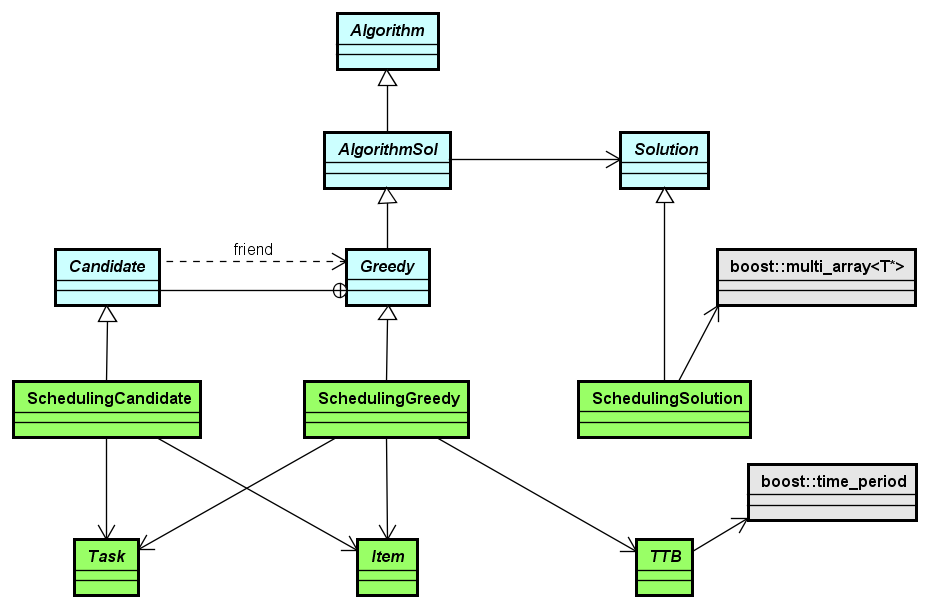
\includegraphics[width=14.9cm,keepaspectratio]{../immagini/progettazione/estensione.png}
        \caption{Architettura generale dell'estensione al framework}
    \end{widepage}
\end{figure}
\FloatBarrier
\noindent
\paragraph{Task} classe che modella un generico \task\ di un problema di scheduling e contiene le strutture dati per salvarne le informazioni relative, ad esempio l'essere aperto/chiuso, o la popolarità.
\paragraph{TTB} classe che modella un generico \ttb\ di un problema di scheduling e contiene le strutture dati per salvarne le informazioni relative, ad esempio gli orari di inizio e fine, o la popolarità.
\paragraph{Item} classe astratta che modella un generico \items\ di un problema di scheduling e contiene le strutture dati per salvarne le informazioni relative, ad esempio gli orari di lavoro, la disponibilità a svolgere straordinari, o la popolarità/fairness che acquisisce man mano che che gli vengono assegnati dei \task. La classe viene approfondita nel paragrafo 6.1 di questo capitolo, relativo alla progettazione di dettaglio.
\paragraph{SchedulingSolution} classe che eredita da \texttt{Solution} e definisce, utilizzando la libreria Boost, un \texttt{multi\textunderscore array<Item*,2>} per salvare lo scheduling prodotto dal metodo \texttt{run()}. Implementa inoltre il metodo \texttt{computeObjective()} calcolando l'obiettivo secondo gli starordinari svolti, la popolarità e la fairness accumulate da tutti gli oggetti di tipo \texttt{Item}.
\paragraph{SchedulingGreedy} classe che eredita da \texttt{Greedy} e ne implementa quindi tutti i metodi virtuali puri. La classe viene approfondita nel paragrafo 6.2 di questo capitolo, relativo alla progettazione di dettaglio.
\paragraph{SchedulingCandidate} classe che eredita da \texttt{Candidate} e modella i candidati da valutare all'interno del metodo \texttt{run()}. Ogni \texttt{SchedulingCandidate} è composto da una coppia \texttt{Item*}, \texttt{Task*} e indica che l'oggetto di tipo \texttt{Task} può essere assegnato all'oggetto di tipo \texttt{Item}.
%**************************************************************
\section{Progettazione dell'applicazione}
Nella \hyperref[fig53]{Figura 5.3} viene presentata l'architettura progettata per la risoluzione del problema del casinò.
\begin{figure}[!h]
    \label{fig53}
    \begin{widepage}
        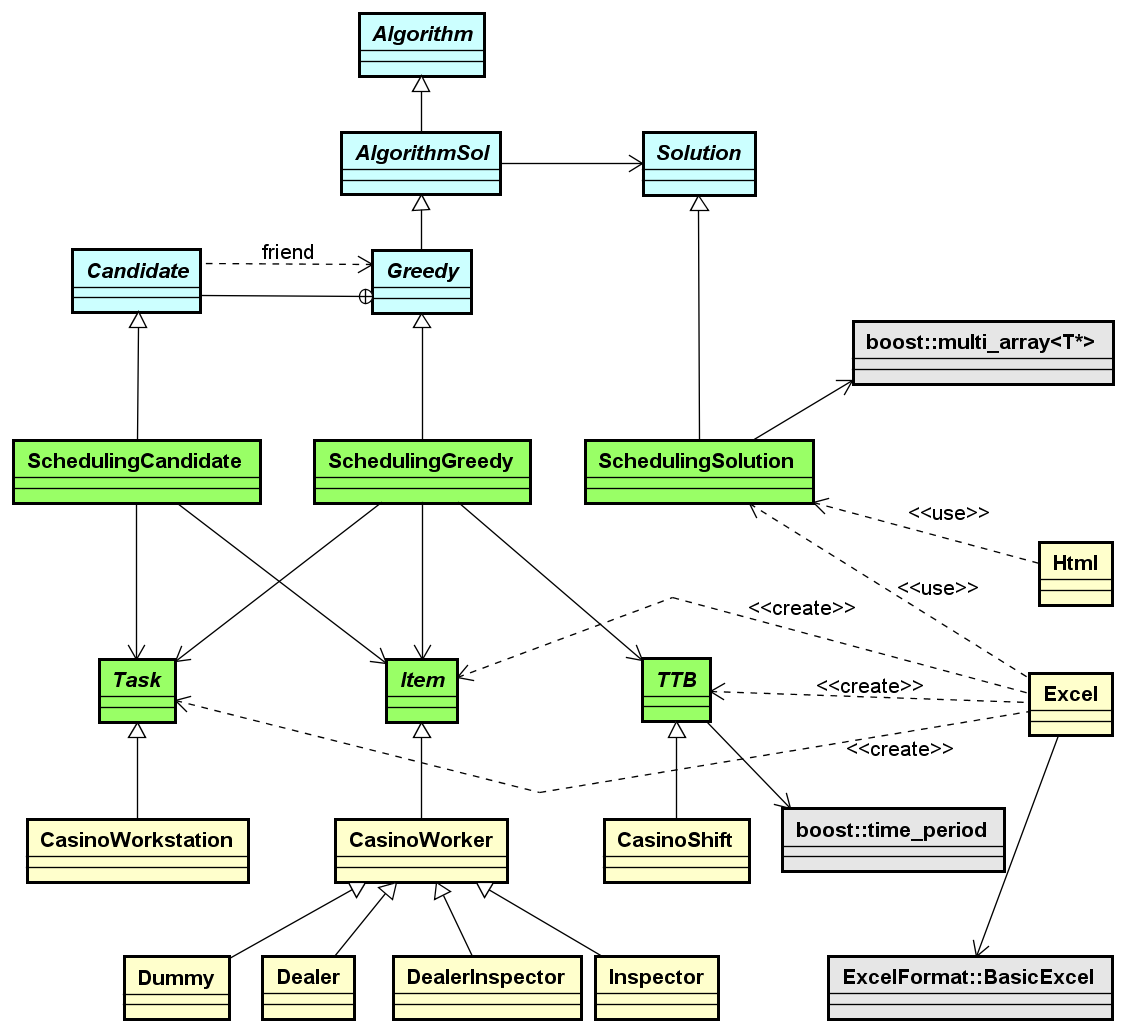
\includegraphics[width=14.9cm,keepaspectratio]{../immagini/progettazione/applicazione.png}
        \caption{Architettura generale dell'applicazione al problema del casinò}
    \end{widepage}
\end{figure}
\FloatBarrier
\noindent
\paragraph{CasinoWorkstation} classe derivata da \texttt{Task}, di cui costituisce una specializzazione. Aggiunge dei campi dati per indicare se la postazione è un tavolo o un pit, il gioco, e il livello.
\paragraph{CasinoShift} classe derivata da \texttt{TTB}, di cui costituisce una specializzazione. Aggiunge un campo dati per indicare il nome del turno.
\paragraph{CasinoWorker} classe derivata da \texttt{Item}, di cui costituisce una specializzazione. Aggiunge dei campi dati per indicare il livello del lavoratore e i giochi da lui conosciuti, oltre a implementare i metodi virtuali puri ereditati da \texttt{Item}. La classe viene approfondita nel paragrafo 6.1 di questo capitolo, relativo alla progettazione di dettaglio.
\paragraph{Dealer} classe derivata da \texttt{CasinoWorker} che modella un dealer.
\paragraph{Inspector} classe derivata da \texttt{CasinoWorker} che modella un inspector.
\paragraph{DealerInspector} classe derivata da \texttt{CasinoWorker} che modella un dealer-inspector.
\paragraph{Dummy} classe derivata da \texttt{CasinoWorker} che modella il Dummy Worker.
\paragraph{Excel} classe che, utilizzando la libreria esterna \texttt{ExcelFormat} si occupa dell'input e output tramite fogli xls.
\paragraph{Html} classe che produce l'output in html.
%*************************************************************
\section{Librerie}
\subsection{ExcelFormat}
ExcelFormat (\citetitle{site:excel}) è una libreria open source che permette di leggere, scrivere e modificare file \emph{\gls{xls}}\glsfirstoccur\ tramite C\texttt{++}. La scelta è ricaduta sull'utilizzare questa libreria per gestire l'input e output in quanto rappresentava un compromesso fra rapidità di programmazione (dato che l'interfaccia utente, come già detto, non era ritenuta prioritaria) e un'interfaccia con un certo grado di controllo dell'input, grazie alle funzioni di Excel, e quanto meno usabile lato utente per inserire gli input e visionare gli output. \\
ExcelFormat offre funzioni per maneggiare i file XLS e i diversi worksheet presenti al loro interno, leggere e scrivere il contenuto delle celle, modificarne la formattazione. Tuttavia le funzioni che offre sono basilari, ad esempio non è possibile scrivere formule.
\subsection{Boost}
Boost  è una collezione di librerie open source che estendono le funzionalità del C\texttt{++}. In particolare, all'interno del progetto sono state usate le librerie:
\begin{itemize}
    \item \textbf{date\textunderscore time:} per gestire orari e date. È stata preferita a \textit{std::time} in quanto offre più funzionalità ed è di utilizzo più immediato.
    \item\textbf{multi\textunderscore array:} per gestire array dinamici multidimensionali. È stata preferita ad annidamenti di contenitori della libreria standard, come \textit{std::vector}, in quanto ne offre un'implementazione più efficiente.
\end{itemize}
%*************************************************************
\section{Design pattern}
\paragraph{Template Method}
\begin{figure}[!h]
    \label{fig54}
    \centering
        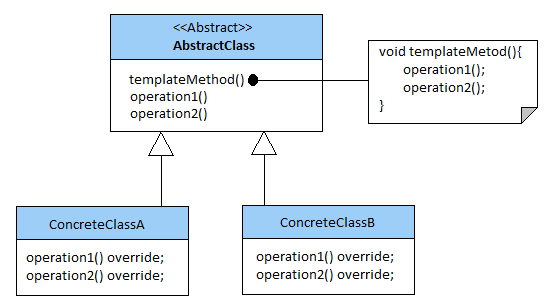
\includegraphics[width=12cm,keepaspectratio]{../immagini/templatemethod.png}
        \caption{Template Method}
\end{figure}
Il Template Method, la cui architettura è presentata nella \hyperref[fig54]{Figura 5.4}, è un design pattern comportamentale che permette di definire lo scheletro di un algoritmo lasciando alle sottoclassi il compito di implementarne alcuni passi come preferiscono. In questo modo si può ridefinire e personalizzare parte del comportamento nelle varie sottoclassi senza dover riscrivere più volte il codice in comune e senza alterarne la struttura. Tale design pattern è stato descritto per la prima volta in \citetitle{gof:dp}.
%**************************************************************

\section{Progettazione di dettaglio}
In questa sezione viene approfondita, tramite diagrammi UML e descrizione dettagliata di classi, metodi e attributi, la progettazione di dettaglio delle classi principali del progetto. Vengono tralasciate le classi più semplici o meno importanti.
\newpage
\subsection{Gerarchia di Item}
Nella \hyperref[fig55]{Figura 5.5} viene presentata la progettazione di dettaglio della gerarchia con classe base \texttt{Item}.
\begin{figure}[!h]
    \label{fig55}
    \begin{widepage}
        \centering
        \includegraphics[width=12cm,keepaspectratio]{../immagini/progettazione/item.png}
        \caption{Gerarchia della classe Item}
    \end{widepage}
\end{figure}
\FloatBarrier
\noindent
\subsubsection{Item}
\begin{itemize}
    \item \textbf{Attributi}
    \begin{itemize}
        \item \texttt{available\textunderscore vec} vettore la cui dimensione è uguale al numero di \ttb. Inizialmente ogni elemento segnala se l'\items\ è disponibile per il \ttb\ (valore -1) o no (valore -2); man mano che l'\items\ viene assegnato ai \task\ durante i \ttb, le celle vengono riempite con gli id dei \task\ svolti.
        \item \texttt{it\textunderscore current} iteratore per available\textunderscore vec, accede all'elemento corrispondente al corrente \ttb.
        \item \texttt{it\textunderscore overtime} iteratore per available\textunderscore vec, accede all'elemento corrispondente al \ttb\ in cui l'\items\ comincia a lavorare gli straordinari.
        \item \texttt{gainedPopularity} tiene memoria della popolarità accumulata dall'\items.
        \item \texttt{gainedFairness} tiene memoria della fairness accumulata dall'\items.
    \end{itemize}
    \item \textbf{Metodi}
    \begin{itemize}
        \item \texttt{getCurrentShift} ritorna l'id del \ttb\ corrente.
        \item \texttt{getConsecutiveShift} calcola e ritorna quanti \ttb\ consecutivi (senza pause) ha lavorato l'\items.
        \item \texttt{howMuchOvertime} calcola e ritorna quanti \ttb\ di straordinari ha lavorato l'\items.
        \item \texttt{addBreak} mette in pausa l'\items\ per il \ttb\ corrente (lascia it\textunderscore current a -1 e lo fa avanzare di uno).
    \end{itemize}
\item \textbf{Metodi virtuali puri}
    \begin{itemize}
        \item \texttt{computePopularity} per calcolare la popolarità accumulata da ogni \items.
        \item \texttt{computeFairness} per calcolare la fairness accumulata da ogni \items.
        \item \texttt{is\textunderscore able} verifica se un \items\ è capace di lavorare ad un certo \task.
        \item \texttt{is\textunderscore available} verifica se un \items\ è disponibile per lavorare ad un certo \task.
        \item \texttt{isQualified} verifica che la mansione di un \items\ sia compatibile con quella richiesta per un \task.
        \item \texttt{assignWorker} per eseguire le operazioni che seguono un assegnamento sull'\items.
    \end{itemize}
\end{itemize}
    
\subsubsection{CasinoWorker}
\begin{itemize}
    \item \textbf{Attributi}
    \begin{itemize}
        \item \texttt{level} è il livello del lavoratore.
        \item \texttt{games} vettore dei giochi conosciuti dal lavoratore.
    \end{itemize}
    \item \textbf{Metodi}
    \begin{itemize}
        \item \texttt{computePopularity} calcola la popolarità accumulata dal lavoratore, tenendo in conto il livello delle postazioni in cui il lavoratore è stato assegnato, quanti turni senza pause ha fatto, quali turni ha fatto e dove.
        \item \texttt{computeFairness} calcola la fairness accumulata dal lavoratore, tenendo in conto se ha lavorato in postazioni dove si siede o si sta in piedi.
        \item \texttt{is\textunderscore able} verifica se il lavoratore è in grado di lavorare in una certa postazione o no, in base alla sua conoscenza del gioco, al livello, alla mansione.
        \item \texttt{is\textunderscore available} verifica se il lavoratore è disponibile a lavorare in una certa postazione, in base non solo alle sue capacità, ma anche dall'essere presente in sala, non dover andare in pausa, non dover rotare di postazione.
        \item \texttt{assignWorker} esegue le operazioni che seguono l'assegnamento del lavoratore: aggiorna available\textunderscore vec e fa avanzare it\textunderscore current, calcola gainedPopularity e gainedFairness.
    \end{itemize}
    \item \textbf{Metodi virtuali puri}
    \begin{itemize}
        \item \texttt{checkLevel} esegue una verifica dell'input riguardante il livello.
        \item \texttt{getLevel} ritorna il livello del lavoratore.
    \end{itemize}
\end{itemize}


\subsubsection{Dealer}
\begin{itemize}
    \item \textbf{Metodi}
    \begin{itemize}
        \item \texttt{checkLevel} controlla che l'input riguardante il livello sia compreso fra 1 e 8. Se sì, ritorna il livello incrementato di due.
        \item \texttt{getLevel} ritorna il livello decrementato di due.
        \item \texttt{isQualified} ritorna true se la postazione è un tavolo, false altrimenti.
    \end{itemize}
\end{itemize}

\subsubsection{Inspector}
\begin{itemize}
    \item \textbf{Metodi}
    \begin{itemize}
        \item \texttt{checkLevel} controlla che l'input riguardante il livello sia compreso fra 1 e 3. Se sì, ritorna il livello.
        \item \texttt{getLevel} ritorna il livello.
        \item \texttt{isQualified} ritorna true se la postazione è un pit, false altrimenti.
    \end{itemize}
\end{itemize}
\subsubsection{DealerInspector}
\begin{itemize}
    \item \textbf{Metodi}
    \begin{itemize}
        \item \texttt{checkLevel} controlla che l'input riguardante il livello sia 3. Ritorna sempre 3.
        \item \texttt{getLevel} ritorna 3.
        \item \texttt{isQualified} ritorna true sia se la postazione è un tavolo, sia se la postazione è un pit.
    \end{itemize}
\end{itemize}
\subsubsection{Dummy}
\begin{itemize}
    \item \textbf{Metodi}
    \begin{itemize}
        \item \texttt{checkLevel} Ritorna sempre 1.
        \item \texttt{getLevel} ritorna 1.
        \item \texttt{isQualified} ritorna sempre true.
        \item \texttt{is\textunderscore available} ritorna sempre true.
    \end{itemize}
\end{itemize}

\subsection{SchedulingGreedy}
Nella \hyperref[fig56]{Figura 5.6} viene presentata la progettazione di dettaglio della gerarchia con classe base \texttt{Greedy}.
\begin{figure}[!h]
    \label{fig56}
    \begin{widepage}
        \centering
        \includegraphics[width=15.5cm,keepaspectratio]{../immagini/progettazione/greedy.png}
        \caption{Gerarchia della classe Greedy}
    \end{widepage}
\end{figure}
\FloatBarrier
\noindent
\begin{itemize}
    \item \textbf{Attributi}
    \begin{itemize}
        \item \texttt{able\textunderscore worker} vettore di liste, ogni elemento del vettore rappresenta un \task\ e i nodi della lista a cui punta sono gli \items\ capaci di svolgere il \task\ (funzione is\textunderscore able). Viene costruito una sola volta e costituisce le coppie \items -\task\ con cui vengono costruiti i candidati.
        \item \texttt{available\textunderscore worker} vettore di liste, ogni elemento del vettore rappresenta un \task\ e i nodi della lista a cui punta sono gli \items\ disponibili a svolgere il \task\ (funzione is\textunderscore available).
        \item \texttt{ordered\textunderscore workstation} vettore dei \task\ ordinati per priorità.
        \item \texttt{currentShift} \ttb\ per il quale l'algoritmo sta schedulando.
    \end{itemize}
    \item \textbf{Metodi}
    \begin{itemize}
        \item \texttt{updateAvailable} aggiorna available\textunderscore worker, eliminando gli \items\ non più disponibili.
        \item \texttt{orderWorkstation} ordina il vettore ordered\textunderscore workstation tramite un counting sort basandosi sul numero di \items\ disponibili per il \task\ (vettore available\textunderscore worker). Il \task\ con meno \items\ disponibili occupa la posizione 0, in fondo al vettore vengono posizionati i \task\ già assegnati.
        \item \texttt{stopConditions} controlla se SchedulingSolution è stata riempita completamente.
        \item \texttt{preprocessCandidates} fa un update di available\textunderscore worker, riordina ordered\textunderscore workstation e poi, basandosi sul \task\ da schedulare come successivo (il primo del vettore) individua il set di candidati da valutare all'interno di candidate\textunderscore list.
        \item \texttt{filterCandidate} controlla che l'\items\ candidato sia disponibile per il \task\ (available\textunderscore workers).
        \item \texttt{ifCandidateFound} chiama assignWorker() sull'\items\ scelto per la schedulazione.
    \end{itemize}
\end{itemize}
%*******************************************************
\section{Codifica e sofware realizzato}
L'implementazione in C\texttt{++} dell'architettura sopra descritta ha prodotto il software desiderato secondo le specifiche fornitemi.\\
Il tutto è stato completato con la scrittura di alcune funzioni in Javascript per rendere più usabile lo scheduling in html fornito in output. In particolare, sono state rese evidenziabili le postazioni all'interno dello scheduling facendoci click sopra; inoltre la prima riga (contente i turni) e la prima colonna (contenente i lavoratori) della tabella dello scheduling sono state rese fisse, in quanto necessariamente la tabella è molto grande e serve quindi uno scroll sia orizzontale che verticale per essere visualizzata per intero.